\documentclass[12pt]{report}
% all imports
\usepackage[utf8]{inputenc}
\usepackage[T1]{fontenc}
\usepackage{lmodern}
\usepackage{amsmath}
\usepackage{hyperref}
\usepackage{booktabs}
\usepackage{bm}
\usepackage[scale=2]{ccicons}
\usepackage[outputdir=build]{minted}
\usepackage{pgfplots}
\usepackage{array,colortbl,xcolor}
\usepgfplotslibrary{dateplot}
\usepackage{setspace}
\usepackage{etoolbox}
\usepackage{xspace}
\usepackage{tikz}
\usetikzlibrary{shapes,arrows,positioning,fit,backgrounds}
\usepackage{tkz-euclide}

\AtBeginEnvironment{quote}{\singlespacing}

% \AtBeginEnvironment{quote}{\singlespacing}

% % new commands
\newcommand{\vect}[1]{\bm{#1}}
\newcommand{\myprime}[1]{{#1}^{\prime}}
\newcommand{\grad}[2]{\nabla_{#1} {#2}}
\newcommand{\dotp}[2]{{#1}^{\top}{#2}}
\newcommand{\dotpPright}[2]{{#1}^{\top}\left({#2}\right)}
\newcommand{\outerp}[2]{\left({#1}\right){#2}^{\top}}
\newcommand{\Jacobian}[2]{\frac{\partial #1}{\partial #2}}
\newcommand{\Vocab}{\mathbb{V}}
 \DeclareMathOperator*{\argmin}{arg\,min}
 \DeclareMathOperator{\E}{\mathbb{E}}

% % definitions
\definecolor{blue}{RGB}{159, 192, 176}
\definecolor{green}{RGB}{160, 227, 127}
\definecolor{orange}{RGB}{243, 188, 125}
\definecolor{red}{RGB}{253, 123, 84}
\definecolor{nephritis}{RGB}{39, 174, 96}
\definecolor{emerald}{RGB}{46, 204, 113}
\definecolor{turquoise}{RGB}{39, 174, 96}
\definecolor{green-sea}{RGB}{22, 160, 133}
\definecolor{purple}{RGB}{181, 124, 215}
% Tikzstyles for Computation Graphs

% nodes
\tikzstyle{noop} = [circle, draw=none, fill=red, minimum size = 10pt]
\tikzstyle{op} = [circle, draw=red, line width=1.5pt, fill=red!70, text=black, text centered, font=\bf \normalsize, minimum size = 25pt]
\tikzstyle{op2} = [circle, draw=orange, line width=1.5pt, fill=orange!70, text=black, text centered, font=\bf \normalsize, minimum size = 25pt]
\tikzstyle{op3} = [circle, draw=orange, line width=1.5pt, fill=orange!70, text=black, text centered, font=\bf \scriptsize, minimum size = 7pt]
\tikzstyle{placeholder} = [circle, draw=red, line width=1.5pt, fill=red!30, text=black, text centered, font=\bf  \normalsize, minimum size = 25pt]
\tikzstyle{state} = [circle, draw=blue, line width=1.5pt, fill=blue!70, text=black, text centered, font=\bf \normalsize, minimum size = 25pt]
\tikzstyle{gradient} = [circle, draw=nephritis, line width=1.5pt, fill=nephritis!60, text=black, text centered, font=\bf \normalsize, minimum size = 25pt]
\tikzstyle{gradient2} = [circle, draw=green2, line width=1.5pt, fill=green2!60, text=black, text centered, font=\bf \normalsize, minimum size = 25pt]
\tikzstyle{textonly} = [draw=none, fill=none, text centered, font=\bf \normalsize]

% edges
% \tikzstyle{tedge}  = [draw, thick, >=stealth, ->]
\tikzstyle{tedge}  = [draw, thick, >=latex, ->]
\tikzstyle{tedge_dashed}  = [draw, thick, >=latex, ->, dashed]

% namedscope
\tikzstyle{namedscope} = [circle, draw=orange, line width=1.5pt, fill=orange!60, align=center, inner sep=0pt]

% \tikzstyle{container} = [draw=none, rectangle, dotted, inner ysep=1.5em]
% \tikzstyle{novertex} = [draw=none, fill=none, text centered]
% \tikzstyle{predicate} = [ellipse, draw, thick, text centered, rounded corners, minimum size=30pt]
% \tikzstyle{aux} = [rectangle, draw, thick, text centered, rounded corners, minimum size=30pt]
% \tikzstyle{ledge}  = [draw, dashed, thick, >=stealth, ->]
% \tikzstyle{pedge}  = [draw, thick, >=stealth, ->]


\title{Adding semantic robustness to dialog agents}
\author{Felipe Salvatore}

\begin{document}

\maketitle

\begin{abstract}
Using the available dataset SICK (Sentence Involving Compositional Knowledge), we introduce a set of new question answering tasks \textbf{Entailment-QA} to measure how well a dialog system deals with abstract semantic knowledge. These tasks force the dialog agent to struggle with distinct notions that are at the intersection of text understanding and reasoning: boolean connectives, first-order quantifiers, synonymy/antinomy/hypernymy resolution, and paraphrase. Experimental results indicate that the current dialog systems present difficulties in solving these tasks.
\end{abstract}
\tableofcontents

\chapter{Introduction}
\label{ch:01-introduction}

One of the main goals in NLP is to build agents capable of \textit{understanding language and reasoning}, i.e., agents capable of carrying a conversation as if they were human. This goal is as old as the field of \textit{artificial intelligence} itself \cite{Turing}, and it is a very ambitious one. We shall call this kind of agents "dialog systems".\\

If we think for a second, there is not a single type of conversation. A dialog between strangers in an elevator, a conversation between one psychologist and his patient, a scientific exchange in a conference; all this can be classified as "dialog" but they present very different dynamics and goals. As a way of refining the analysis, the NLP literature on dialog made the distinction between \textit{goal-driven dialog systems} and \textit{non-goal-driven dialog systems}; the former includes \textit{chatbots}, normally used in the industry for technical support services or information acquisition; the latter is a term used to refer to any conversational agent with no explicit purpose.

Each paradigm presents its advantages and disadvantages: on the one hand goal-driven dialog systems are useful systems but they demand a precise understanding (of the goal at hand) and there are not so much available data to train a goal-driven agent. On the other hand, non-goal-driven dialog systems produce, at best, chit-chat conversation. So is not so easy to justify it's relevancy and at the same time he have a lot of available data to train such models (movie legends, social media conversations, etc.). 

There is a central difference between these two paradigms, although non-goal-driven systems may seen interesting for its comprehensiveness, it presents a central problem: \textit{there is no good quantitative metric to compare non-goal-driven agents}, and as a consequence \textit{there is also no standardized benchmark}. We can frame the dialog task between two agents A and B as a translation problem: the source language is the set of utterances spoken by A, similarly, the target language is the sentences of B. Then, the dialog system is just a program translating massages from A to B. So it makes sense to consider the use of quantitative metrics for automatic translation, metrics like BLUE \cite{Papineni02bleu:a} and METEOR \cite{Lavie:2007:MAM:1626355.1626389}. But as pointed out by \cite{LiuLSNCP16, LoweSNCP16}, regarding dialog, \textit{these metrics correlate very weakly with human judgement}.

A more fruitful approach is the one from the goal-driven systems literature: developed a series of synthetic tasks in the form of question answering (QA) to test different capabilities of the competing models \cite{BordesW16, Hixon15, WestonBCM15}. Each task tries to assert one prerequisite to full language understanding.

Here we propose to expand the work done in \cite{BordesW16, WestonBCM15} by \textit{adding new testbeds for complex semantic relationships}: \textbf{Entailment-QA}. The motivation behind this expansion is to guarantee that an end-to-end machine learning model can perform \textit{complex linguistic inferences}. We focus on two kind of inferences: the ones defined by \textit{logical operators} and others defined by \textit{word knowledge}.


\section{Motivation}
\label{sec:motivation}

Logic is not important by itself, but it can help us build agents capable of distinguishing between sentences that have a real informational content from sentences that do not. A rational agent should be able to spot contradictions in a sentence. Although this importance, logical reasoning is one area that is often neglected by Conversational AI researchers. This Ph.D. proposal is one step towards a more elaborate analysis.

An intelligent agent should distinguish between \textit{meaningful} and \textit{nonsensical} speech. To do that the agent can make use of background knowledge, but it can also point out \textit{gaps in the speech's rationality}. Logic is the study of reasoning. Over the time it became a complex discipline with its own concepts, tools and language. Here we will use some logical notions like \textit{entailment} and \textit{contradiction} to build a set of synthetic tasks. All tasks presented are focused on the distinction between \textit{sound} and \textit{unsound} speech. The difference between tasks resides in the use of certain semantic structures.



% ------------------------------------------------------------------------
\section{Objectives}
\label{sec:objectives}

The main objective of this research project is to propose a new set of synthetic tasks in the same lines as \cite{WestonBCM15} in order to help evaluating and building dialog systems that present reasonable text reasoning capabilities.


% ------------------------------------------------------------------------
\section{Organization}
\label{sec:organization}

Chapter 2 exposes the theory that is the basis for the research. Chapter 3 presents our proposed task to evaluate logical reasoning. Chapter 4 describe the proposed methodology. And chapter 5 discuss the possible results of this research.




\chapter{Background}
\label{ch:02-background}


\section{Machine Learning}


\section{Neural Networks}


A neural network is a non-linear function $f(\vect{x}; \theta)$. It is defined by a collection of parameters $\vect{\theta}$ and a collection of non-linear transformations. It is usual to represent $f$ as a compositions of functions:

\begin{align}
f(\vect{x}; \theta) &= f^{(2)}(f^{(1)}(\vect{x}; \vect{W}_1, \vect{b}_1); \vect{W}_2, \vect{b}_2)\\
&= softmax(\vect{W}_2 (\sigma(\vect{W}_1\vect{x} + \vect{b}_1)) + \vect{b}_2)
\end{align}


The output of these intermediary functions are referred as \textit{layers}. So in the example above, $\vect{x}$ (the output of the identity function) is the \textit{input layer}, $f^{(1)}(\vect{x}; \vect{W}_1, \vect{b}_1)$ is the \textit{hidden layer} and $f^{(2)}(f^{(1)}(\vect{x}; \vect{W}_1, \vect{b}_1); \vect{W}_2, \vect{b}_2)$ is the \textit{output layer}. Since each layer is a vector, we normally speak about the \textit{dimension} of a layer. For historical reasons we also say that each entry on a layer is a \textit{node} or a \textit{neuron}.  Models with a large number of hidden layers are called \textit{deep models}, for this reason the name \textit{deep learning} is used.  

\par A neural network is a function approximator: it can approximate any Borel measurable function from one finite dimensional space to another with any desired nonzero amount of error. This theoretical result is know as the \textit{universal approximation theorem}\cite{Cybenko}. Without entering in the theoretical concepts, it suffice to note that the family of Borel mensurable functions include all continuous functions on a closed and bounded subset of $\mathbb{R}^n$.



Different deep learning architectures are used in NLP: \textit{convolutional architectures} have a good performance in tasks were it is required to find a linguistic indicator regardless of its position (e.g., document classification, short-text categorization, sentiment classification, etc); high quality word embeddings can be achieved with models that are a kind of \textit{feedforward neural network} \cite{Mikolov23}. But for a variety of works in natural language we want to capture regularities and similarities in a text structure. That is way \textit{recurrent} and \textit{recursive} models have been widely used in the field. Here we are focused on generative models and since recurrent models have been producing very strong results for language modeling \cite{goldberg15}, we will concentrate on them.

\section{Recurrent Neural Network}
\label{sec:RNN}


\textit{Recurrent neural network} (RNN) is a family of neural network specialized in sequential data $\vect{x}_1, \dots, \vect{x}_\tau$. As a neural network, a RNN is a parametrized function that we use to approximate one hidden function from the data. As before we can take the simplest RNN as a neural network with only one hidden layer. But now, what make RNNs unique is a recurrent definition of one of its hidden layer:

\begin{equation}
\vect{h}^{(t)} = g(\vect{h}^{(t-1)}, \vect{x}^{(t)}; \vect{\theta})
\end{equation}

$\vect{h}^{(t)}$ is called \textit{state}, \textit{hidden state}, or \textit{cell}.


\par This recurrent equation can be unfolded for a finite number of steps $\tau$. For example, when $\tau =3$:
\vspace{0.2cm}

\begin{align}
\vect{h}^{(3)}& = g(\vect{h}^{(2)}, \vect{x}^{(3)}; \vect{\theta})\\
 & = g(g(\vect{h}^{(1)}, \vect{x}^{(2)}; \vect{\theta}), \vect{x}^{(3)}; \vect{\theta})\\
 & = g(g(g(\vect{h}^{(0)}, \vect{x}^{(1)}; \vect{\theta}), \vect{x}^{(2)}; \vect{\theta}), \vect{x}^{(3)}; \vect{\theta})\\
\end{align}

Using a concret example consider the following classification model define by the equations:

\begin{equation}
f(\vect{x}^{(t)}, \vect{h}^{(t-1)}; \vect{V}, \vect{W}, \vect{U}, \vect{c}, \vect{b}) = \vect{\hat{y}}^{(t)}
\end{equation}
 \vspace{0.2cm}
\begin{equation}
\vect{\hat{y}}^{(t)} = softmax(\vect{V} \vect{h}^{(t)} + \vect{c})
\end{equation}
\vspace{0.2cm}
 \begin{equation}
\vect{h}^{(t)} = g(\vect{h}^{(t-1)}, \vect{x}^{(t)}; \vect{W},\vect{U}, \vect{b})
\end{equation}
\vspace{0.2cm}
\begin{equation}
\vect{h}^{(t)} = \sigma(\vect{W} \vect{h}^{(t-1)} + \vect{U} \vect{x}^{(t)} + \vect{b})
\end{equation}

This kind of model can create an output $\vect{\hat{y}}^{(t)}$ at each time $t$, or the model can produce a single output $\vect{\hat{y}}$ after processing an entire input sequence. This choice depends on the learning problem that is being modeled.

With the model's prediction at hand, we can use a loss function (like cross entropy for the classification problem) and apply the back-propagation algorithm to optimize the model. These models look complex, but it quite straightforward to compute the gradients \cite[p.~374]{DeepLearningbook}.

Although this kind of deep learning model is very useful, it presents a severe flaw. When computing the gradients there is a lot of repeated matrix multiplication using the recurrent weight matrix (in the example above, the matrix $\vect{W}$). Depending on some configurations of this matrix \textit{the gradients may vanish or explode exponentially with respect to the number of time steps}.

Thus, handing long-term dependencies became a problem when using RNNs. Different solutions were proposed, the most effective results came from some modifications of this model. We will present the two most famous modifications: the gated recurrent unit and the long short-term memory. 

\section{Gated Recurrent Unit}
\label{sec:GRU}

To capture long-term dependencies on a RNN  the authors of the paper \cite{ChungGCB14}  proposed a new architecture called \textit{gated recurrent unit} (GRU). This model was constructed to make each hidden state  $\vect{h}^{(t)}$ to adaptively capture dependencies of different time steps. It work as follows, at each step $t$ one candidate for hidden state is formed:

\begin{equation}
\vect{\widetilde{h}}^{(t)} = tahn(\vect{W} (\vect{h}^{(t-1)} \odot  \vect{r}^{(t)}) + \vect{U} \vect{x}^{(t)} + \vect{b})
\end{equation}


where $\vect{r}^{(t)}$ is a vector with values in $[0, 1]$ called a \textit{reset gate}, i.e.,  a vector that at each entry outputs the probability of reseting the  corresponding entry in the previous hidden state $\vect{h}^{(t-1)}$. Together with $\vect{r}^{(t)}$ we define an \textit{update gate}, $\vect{u}^{(t)}$. It is also a vector with values in $[0, 1]$. Intuitively we can say that this vector decides how much on each dimension we will use the candidate update. Both $\vect{r}^{(t)}$ and $\vect{u}^{(t)}$ are defined by $\vect{h}^{(t-1)}$ and $\vect{x}^{(t)}$; they also have specific parameters:

\begin{equation}
\vect{r}^{(t)} = \sigma(\vect{W}_{r} \vect{h}^{(t-1)} + \vect{U}_{r} \vect{x}^{(t)} + \vect{b}_{r})
\end{equation}


\begin{equation}
\vect{u}^{(t)} = \sigma(\vect{W}_{u} \vect{h}^{(t-1)} + \vect{U}_{u} \vect{x}^{(t)} + \vect{b}_{u})
\end{equation}

At the end the new hidden state $\vect{h}^{(t)}$ is defined by the recurrence:

\begin{equation}
\vect{h}^{(t)} = \vect{u}^{(t)} \odot \vect{\widetilde{h}}^{(t)} + (1 - \vect{u}^{(t)}) \odot \vect{h}^{(t-1)} 
\end{equation}

Note that the new hidden state combines the candidate hidden state $\vect{\widetilde{h}}^{(t)}$ with the past hidden state $\vect{h}^{(t-1)}$ using both $\vect{r}^{(t)}$ and $\vect{u}^{(t)}$ to adaptively copy and forget information.

\section{Long Short-Term Memory}
\label{sec:LSTM}


\textit{Long short-term memory} (LSTM) is one of the most applied versions of the RNN family of models. Historically it was developed before the GRU model, but conceptually we can think in the RNN as an expansion of the model presented in the last session. Because of notation differences they can look different. LSTM is also based on parametrized gates; in this case three: the \textit{forget gate}, $\vect{f}^{(t)}$, the \textit{input gate}, $\vect{i}^{(t)}$, and the \textit{output gate}, $\vect{o}^{(t)}$. The gates are defined only by $\vect{h}^{(t-1)}$ and $\vect{x}^{(t)}$ with specific parameters:

\begin{equation}
\vect{f}^{(t)} = \sigma(\vect{W}_{f} \vect{h}^{(t-1)} + \vect{U}_{f} \vect{x}^{(t)} + \vect{b}_{f})
\end{equation}

\begin{equation}
\vect{i}^{(t)} = \sigma(\vect{W}_{i} \vect{h}^{(t-1)} + \vect{U}_{i} \vect{x}^{(t)} + \vect{b}_{i})
\end{equation}

\begin{equation}
\vect{o}^{(t)} = \sigma(\vect{W}_{o} \vect{h}^{(t-1)} + \vect{U}_{o} \vect{x}^{(t)} + \vect{b}_{o})
\end{equation}

Intuitively $\vect{f}^{(t)}$ should control how much informative will be discarded, $\vect{i}^{(t)}$ controls how much information will be updated, and $\vect{o}^{(t)}$ controls how munch each component should be outputted. A candidate cell, $\tilde{\vect{c}}^{(t)}$ is formed:

\begin{equation}
\tilde{\vect{c}}^{(t)} = tahn(\vect{W} \vect{h}^{(t-1)} + \vect{U} \vect{x}^{(t)} + \vect{b})
\end{equation}

and a new cell $\tilde{\vect{c}}^{(t)}$ is formed by forgetting some information of the previous cell $\tilde{\vect{c}}^{(t-1)}$ and by adding new values from $\tilde{\vect{c}}^{(t)}$ (scaled by the input gate)

\begin{equation}
\vect{c}^{(t)} = \vect{f}^{(t)} \otimes \vect{c}^{(t-1)} + \vect{i}^{(t)}\otimes \tilde{\vect{c}}^{(t)}
\end{equation}

The new hidden state, $\vect{h}^{(t)}$, is formed by filtering $\vect{c}^{(t)}$:

\begin{equation}
\vect{h}^{(t)} = \vect{o}^{(t)} \otimes tanh(\vect{c}^{(t)})
\end{equation}


Until now we have presented general deep learning theory, now we will focus on the specificities of these models applied to natural language problems.


\section{Language model}

We call \textit{language model} a probability distribution over sequences of tokens in a natural language.

\[
P(x_1,x_2,x_3,x_4) = p
\]

This model is used for different nlp tasks such as speech recognition, machine translation, text auto-completion, spell correction, question answering, summarization and many others.

The classical approuch to a languange model was to use the chain rule and a markovian assumptiom, i.e., for a specific $n$ we assume that:

\begin{equation}
P(x_1, \dots, x_T) = \prod_{t=1}^{T} P(x_t \vert x_1, \dots, x_{t-1}) = \prod_{t=1}^{T} P(x_{t} \vert x_{t - (n+1)}, \dots, x_{t-1})
\end{equation} 


This gave raise to models based on $n$-gram statistics. The choice of $n$ yields different models; for example 
\textit{Unigram} language model ($n=1$): 
\begin{equation}
P_{uni}(x_1, x_2, x_3, x_4) = P(x_1)P(x_2)P(x_3)P(x_4)
\end{equation}

where $P(x_i) = count(x_i)$.\\

\textit{Bigram} language model ($n=2$): 
\begin{equation}
P_{bi}(x_1,x_2,x_3,x_4) = P(x_1)P(x_2\vert x_1)P(x_3\vert x_2)P(x_4\vert x_3)
\end{equation} 
where
\[
P(x_i\vert x_j) = \frac{count(x_i, x_j)}{count(x_j)}
\]


Higher $n$-grams yields better performance. But at the same time higher $n$-grams requires a lot of memory\cite{Heafield}.

Since \cite{Mikolov11} the approach has change, instead of using one approach that is specific for the language domain, we can use a general model for sequential data prediction: a RNN.

So, our learning task is to estimate the probability distribution 

\[
P(x_{n} = \text{word}_{j^{*}} | x_{1}, \dots ,x_{n-1})
\]

for any $(n-1)$-sequence of words $x_{1}, \dots ,x_{n-1}$.

We start with a corpus $C$ with $T$ tokens and a vocabulary $\Vocab$.\\\

Example: \textit{Make Some Noise} by the Beastie Boys.\\

\begin{quote}
Yes, here we go again, give you more, nothing lesser\\
Back on the mic is the anti-depressor\\
Ad-Rock, the pressure, yes, we need this\\
The best is yet to come, and yes, believe this\\
... \\
\end{quote}

\begin{itemize}
\item $T = 378$
\item $|\Vocab| = 186$
\end{itemize}


The dataset is a collection of pairs $(\vect{x},\vect{y})$ where $\vect{x}$ is one word and $\vect{y}$ is the immediately next word. For example:
\begin{itemize}
\item [] $(\vect{x}^{(1)}, \vect{y}^{(1)}) =$ (Yes, here).
\item [] $(\vect{x}^{(2)}, \vect{y}^{(2)}) =$ (here, we)
\item [] $(\vect{x}^{(3)}, \vect{y}^{(3)}) =$ (we, go)
\item [] $(\vect{x}^{(4)}, \vect{y}^{(4)}) =$ (go, again)
\item [] $(\vect{x}^{(5)}, \vect{y}^{(5)}) =$ (again, give)
\item [] $(\vect{x}^{(6)}, \vect{y}^{(6)}) =$ (give, you)
\item [] $(\vect{x}^{(7)}, \vect{y}^{(7)}) =$ (you, more)
\item [] $\dots$
\end{itemize}

Notation

\begin{itemize}
\item $\vect{E} \in \mathbb{R}^{d,|\Vocab|}$ is the matrix of word embeddings.
\vspace{0.3cm}
\item $\vect{x}^{(t)} \in \mathbb{R}^{|\Vocab|}$ is one-hot word vector at time step $t$.
\vspace{0.3cm}
\item $\vect{y}^{(t)} \in \mathbb{R}^{|\Vocab|}$ is the ground truth at time step $t$ (also an one-hot word vector).
\end{itemize}

The language model is similar as the RNN described above. It is defined by the following equations:

\begin{equation}
\vect{e}^{(t)} = \vect{E}\vect{x}^{(t)}
\end{equation}
\vspace{0.2cm}
 \begin{equation}
\vect{h}^{(t)} = \sigma(\vect{W}\vect{h}^{(t-1)}+ \vect{U}\vect{e}^{(t)}+ \vect{b})
\end{equation}
\vspace{0.2cm}
\begin{equation}
\vect{\hat{y}}^{(t)} = softmax(\vect{V}\vect{h}^{(t)} + \vect{c})
\end{equation}



At each time $t$ the point-wise loss is:

\vspace{0.2cm}

\begin{align}
L^{(t)} &= CE(\vect{y}^{(t)},\vect{\hat{y}}^{(t)})\\
    &= - \log(\vect{\hat{y}}_{j^{*}})\\
        &= - \log P(x^{(t+1)} = \text{word}_{j^{*}}|x^{(1)}, \dots, x^{(t)})
\end{align}

The loss $L$ is the mean of all the point-wise losses
\begin{equation}
L=\frac{1}{T}\sum_{t=1}^{T}L^{(t)}
\end{equation}


Evaluating a language model. We can evaluate a  language model using a \textit{extrinsic evaluation}: How our model perform in a NLP task such as text auto-completion. Or a \textit{intrinsic evaluation}: Perplexity (PP) can be thought as the weighted average branching factor of a language.


Given $C= x_1, x_2, \dots, x_T$, we define the perplexity of $C$ as:

\begin{align}
PP(C) &= P(x_1, x_2, \dots, x_T)^{-\frac{1}{T}}\\
    & \\
      &= \sqrt[T]{\frac{1}{P(x_1, x_2, \dots, x_T)}}\\
      & \\
      &= \sqrt[T]{\prod_{i=1}^{T}\frac{1}{P(x_i \vert x_1,\dots, x_{i-1})}}
\end{align}

we can relate Loss and Perplexity:

Since
\begin{align}
L^{(t)} & = - \log P(x^{(t+1)} |x^{(1)}, \dots, x^{(t)})\\
& =  \log(\frac{1}{P(x^{(t+1)}|x^{(1)}, \dots, x^{(t)})})\\
\end{align}
We have that:

\begin{align}
        L &=\frac{1}{T} \sum_{t=1}^{T} L^{(t)}\\
          &= \log\left( \sqrt[T]{\prod_{i=1}^{T}\frac{1}{P(x_i \vert x_1,\dots, x_{i-1})}} \right)\\
          &= \log(PP(C))
\end{align}

So another definition of perplexity is

\begin{equation}
2^{L} = PP(C)
\end{equation}





\section{Seq2seq}
\label{sec:Seq2seq}

fsdfdsfdsf



\section{Atention}
\label{sec:Atention}

fksdhfjsdgjf


\chapter{Dialog Systems}
\label{ch:03-dialog-systems}


\section{Using neural networks to generate dialog}
\label{ch:03-gen}

Sequence to sequence models are originally formulated to improve the automatic translation task [ref]. The authors of \cite{DBLP:journals/corr/VinyalsL15} proposed to use this model for generating dialog, and since then the field of dialog generation was revolutionized. As we have seen, a seq2seq model encodes the source sentence in a vector $\vect{h}$ and uses this vector to initiate a language model.

This can be used to model a dialog as follows: suposse we have recorded two agents A and B. We will use this dialog as the training data for our model. The model will try to predict how B would respond. Let $\vect{s} = s_1, s_2, \dots, s_n$ be an utterance from A and  $\vect{x} = x_1, x_2, \dots, x_m$ be the response from B (both $\vect{s}$ and $\vect{x}$ are a sequence of words). $\vect{s}$ is input to an encoder network, which is a RNN. The encodes summarizes the input utterance into a vector, say $\vect{h}$, and this vector is used to initiate the decoder model, which is another RNN. And the decoder takes as input $\vect{x}$ and at each time $t$ the model tries to predict the word $t+1$ using $x_1, x_2, ...., x_{t-1}, \vect{h}$. This became a multiclass classification task, and we train the model by minimizing the cross entropy loss.


After we training we can use the same model to generate a new dialog: the agent A gives an utterance ans we use the encoder model to summarize this uterance in a vector h as before, but now we use the probability distribution learned by the decoder model (initialized by $\vect{h}$) to sample words until it generates an end-of-speech <eos> token (or until a upper bound for the uterance size is reached). This approach allows for variable length inputs and outputs.

This is the base for more complex models. For example, take the hierarchical recurrent encoder-decoder architecture (HRED) proposed by Sordoni et al. \cite{Serban:2016a}. In this setting a dialogue is viewed as a sequence of utterances $D=\langle U_1 , \dots, U_M \rangle$ involving two interlocutors such that each $U_i$ contains a sequence of $N_i$ tokens, $U_i = \langle w_{i,1} , \dots, w_{i,N_{i}} \rangle$. Each $w_{i,j}$ is a random variable that taking values in the $V\cup A$ where $V$ is the vocabulary and $A$ is the set of \textit{speech acts} (for example 'pause' and 'end of turn' are  speech acts). In this case the learning task is the same as the one in language modeling: we want to estimate of the probability of one token (speech acts included) conditioned on the previously tokens:

\begin{equation}
P(w_{i,j} | w_{i,1}, \dots , w_{i,j-1}, U_{1}, \dots U_{i-1})
\end{equation}

The different dialogues $\langle U_1 , \dots, U_M \rangle$ will serve as a corpus.
In this paper the authors use a \textbf{Hierarchical Recurrent Encoder-Decoder model(HRED)}, i.e., a model based on three RNNs: an \textit{encoder} RNN, a \textit{context} RNN and a \textit{decoder} RNN.  To understand the workings of this model, suppose we have the following dialog:
\begin{itemize}
\item ($U_1$) Mom, I don't feel so good.\\
\item ($U_2$) What's wrong?\\
\item ($U_3$) I feel like I'm going to pass out.
\end{itemize}

First the encoder RNN will encode the sentence $U_1$ in a vector $\vect{U}_1$, then the context RNN will compute a hidden state, say $\vect{C_1}$ using $\vect{U}_1$ and all past sentences in the dialog. After that the decoder RNN will use $U_2$ as an input to predict the next word using $\vect{C_1}$. The same procedure is repeated for $U_2$. Figure
x shows the computational graph of this process.

\begin{figure}[ht!]
\label{HRED}
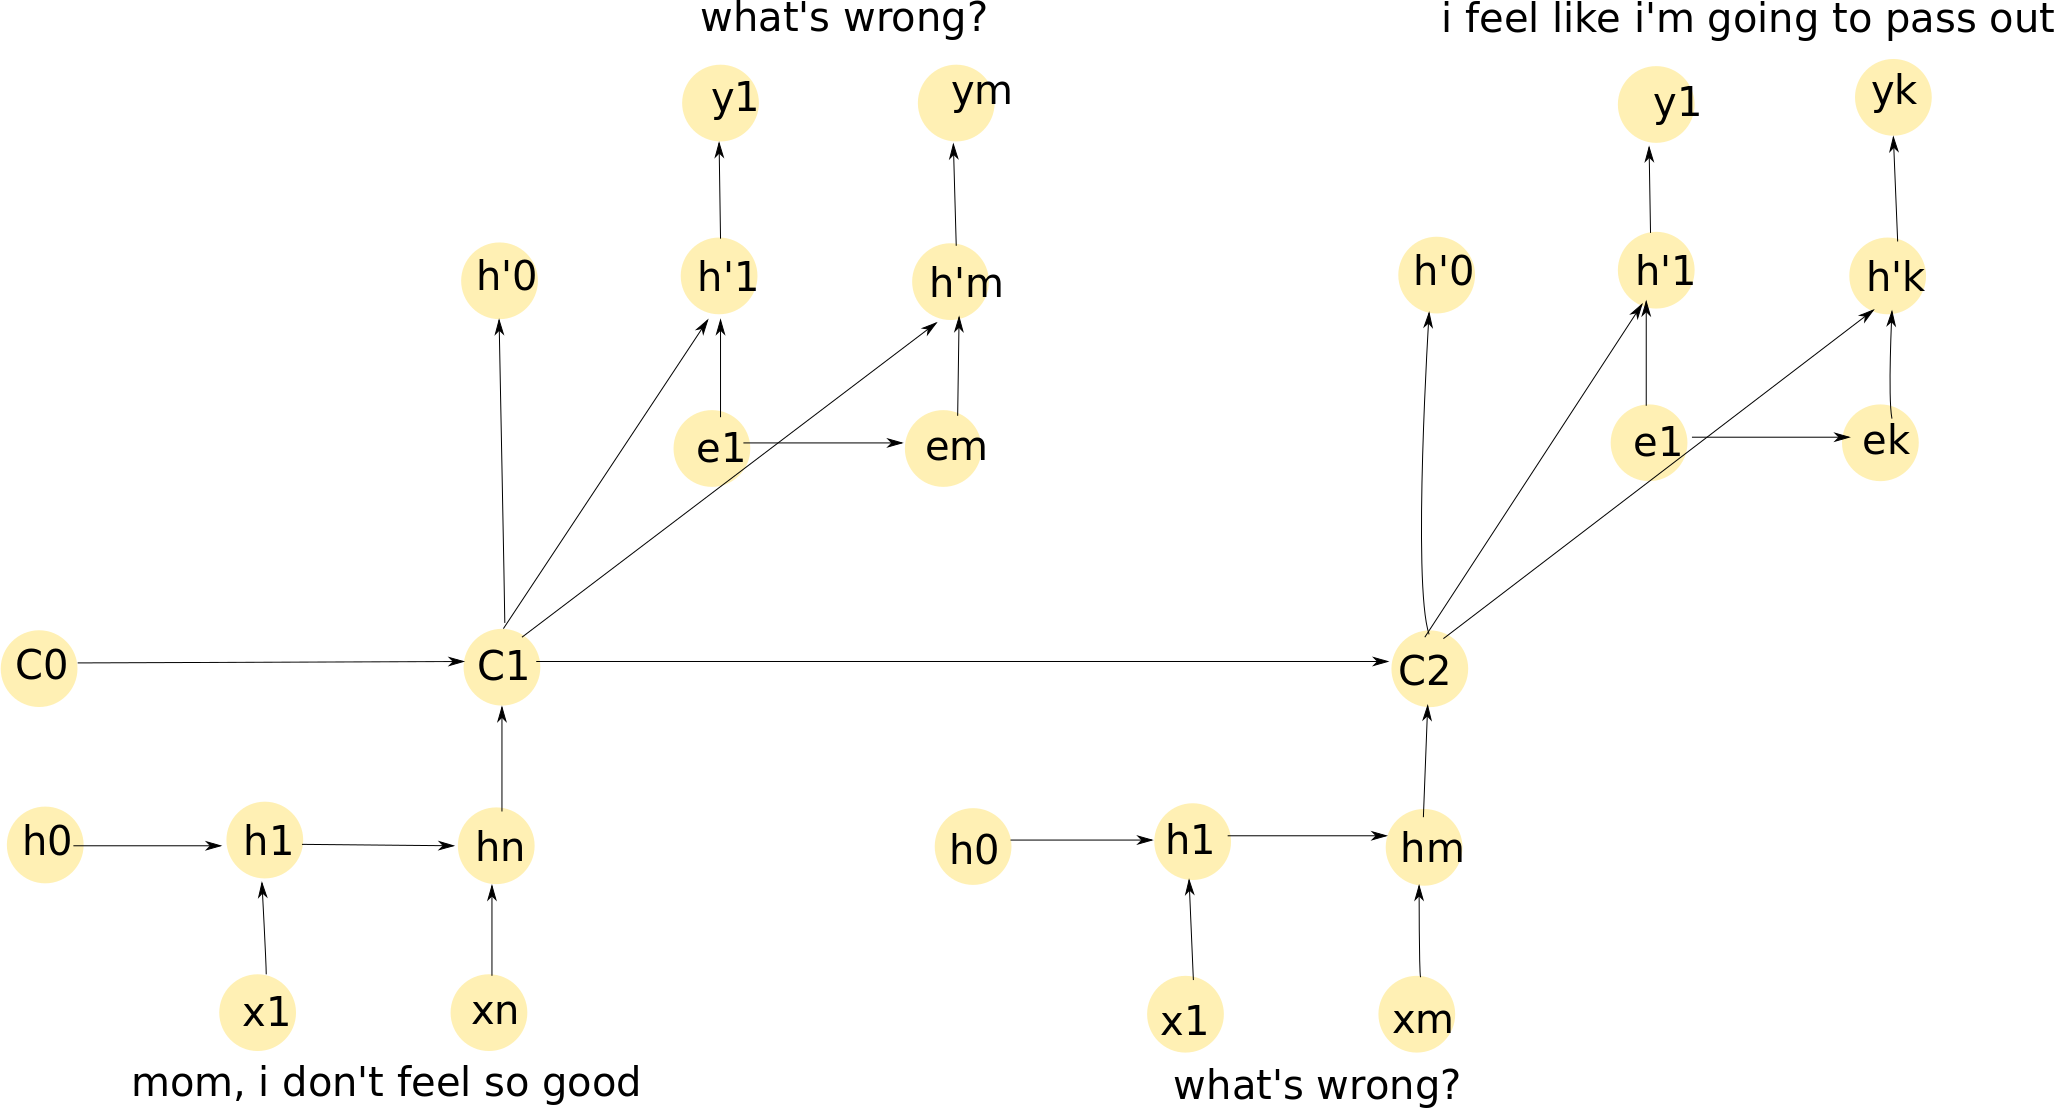
\includegraphics[width=10cm]{img/HRED_placeholder.png}
\caption{HRED model}
\end{figure}

Note that in this model the prediction is conditioned on the hidden state of the context RNN.



\section{How to evaluate dialogs?}

\label{ch:03-eval}

In the seminal paper by Alan Turing \cite{Turing} it is proposed a game to evaluate a dialog system. The idea behind the game was simple: three players A, B and C can interact only by nonpersonal communication. C knows that he will interact with a dialog system (A) and a person (B), but he does not know which is which. C should exchange some conversation both with A and B; after some time he should guess who is the dialog system and who is the human. The goal of A is to be as human as possible in order to fool C; and the goal of B is to help C come to the right answer.

\par This is the famous \textit{Turing Test}. If the dialog system wins this game we say that \textit{it has passed the Turing Test}. For many people this is the holy grail of artificial intelligence. We disagree with that. [Give your oppion about that]


\subsection{Human evaluation}

The most basic form to check if a generated sentence is sound is by using human evaluations. Hence is normal to see researches making use of crowdsourced judges (using services like Amazon Mechanical Turk). These judges can say that a generated sentence is just good or bad, in an informal way. But we can also use a more rigorous score system. 



In \cite{Stent} the authors enumerate three criteria to judge a generated sentence:

\begin{enumerate}
\item \textit{adequacy}: the meaning equivalence between the generated and control sentence. 
\item \textit{fluency}: the syntactic correctness of the generated sequence.
\item \textit{readability}: efficacy of the generated sentence in a particular context.
\end{enumerate}


\subsection{BLUE}
This metric was proposed in \cite{Papineni2001} for automatic translation. It compares n-grams (up to 4) of the candidate translation with the n-grams of the reference translation and count the number of matches; it also ads brevity penalty for too short translations. The formula for this metrics is:

\begin{equation}
BLUE = min \left(1, \frac{output-length}{reference-lenght} \right) \left(\prod_{n=1}^{4} precision_{n} \right)^{\frac{1}{4}}
\end{equation}

Where $precision_{n}$ is number of $n$-gram overlap between the candidate and the reference divided by the number of all $n$-grams in the candidate. BLUE scores ranges from $0$ to $1$. Typically this score is computed over an entire corpus and was originally designed for use with multiple reference sentences. To give one simple example we will use the following Portuguese sentence:

\begin{center}
`em plano aberto, a cidade parece linda'
\end{center}

The reference translation is

\begin{center}
`in a wide shot, the city looks beautiful'
\end{center}

Now consider two candidates:

\begin{center}
$c_1$: `in the open, the city looks beautiful'\\
$c_2$: `in open plan, the city looks gorgeous'\\
\end{center}

\begin{figure}
\label{bluetable}
\begin{center}
\begin{tabular}{|c|c|c|}
\hline
\cellcolor{blue!10} Metric& \cellcolor{blue!10} $c_1$ & \cellcolor{blue!10} $c_2$ \\ \hline
\cellcolor{blue!10} $precision_1$& $5/7$ & $4/7$ \\ \hline
\cellcolor{blue!10} $precision_2$& $3/6$ & $2/6$  \\ \hline
\cellcolor{blue!10} $precision_3$& $2/5$ & $1/5$  \\ \hline
\cellcolor{blue!10} $precision_4$& $1/4$ & $0/4$  \\ \hline
\cellcolor{blue!10} brevity penalty& $7/8$ & $7/8$  \\ \hline
\cellcolor{blue!10} $BLUE$& $0.38$ & $0$ \\ \hline
\end{tabular}
\end{center}
\end{figure}


Table \ref{bluetable} shows the precision for each $n$-gram (up to $4$) and the BLUE score for each candidate.

\section{Creating simplified tasks}
\label{ch:03-tasks}

Speak about bAbI


\section{The logical entailment problem inside the bAbI task}
\label{ch:03-tasks}


In \cite{WestonBCM15}, among a variety of useful tasks the authors introduce two tasks that deals with logical inference: \textit{basic deduction} and \textit{basic induction}. The basic deduction task offers questions of the form:

\begin{quote} 
\centering 
$P^{1}$ are afraid of $Q^{1}$\\
$P^{2}$ are afraid of $Q^{2}$\\
$P^{3}$ are afraid of $Q^{3}$\\
$P^{4}$ are afraid of $Q^{4}$\\
$c^{1}$ is a $P^{1}$\\
$c^{2}$ is a $P^{2}$\\
$c^{3}$ is a $P^{3}$\\
$c^{4}$ is a $P^{4}$\\
What is $c^j$ afraid of? A: $P^{j}$\\
\end{quote}

where $P^j$ and $Q^j$ are animals (e.g., "cats", "mice", "wolfs", etc.) and $c^j$ are names (e.g., "Jessica", "Gertrud", "Emily", etc.). The underlying relation under focus here is the \textit{membership} relation: if Emily is a cat and cats are afraid of wolfs then Emily is afraid of wolfs. This task is solvable by the current models, in \cite{WestonBCM15} the best accuracy for this task is $100\%$. 

The basic induction task is composed by questions of the form:

\begin{quote} 
\centering 
$c^{1}$ is a $P^{1}$\\
$c^{1}$ is $C^{1}$\\
$c^{2}$ is a $P^{2}$\\
$c^{2}$ is $C^{2}$\\
$c^{3}$ is a $P^{3}$\\
$c^{3}$ is $C^{3}$\\
$c^{4}$ is a $P^{4}$\\
$c^{4}$ is $C^{4}$\\
$c$ is a $P^{j}$\\
What color is $c$? A: $C^{j}$\\
\end{quote}

Where $P^{j}$ is a animal, $C^{j}$ is a color, and $c^{j}$ is a name. Here the agent is asked to remember the relation between animal and color, and when presented a new name of an animal in the example, the agent should infer the color using past examples. Similar to the deduction task, in \cite{WestonBCM15} is reported that this task is completely solved.

These two tasks present a first step towards \textit{a complete set of tasks to tests inference capabilities}. One aspect that is missing though is the use of logical operators such as \textit{boolean connectives} and \textit{first-order quantifiers}. Those operators play a big role on everyday speech, hence a natural way of expanding this work is by creating a set of tasks that make agents learn \textit{valid logic structures}.

\section{Entailment-QA}
\label{ch:03-EQA}

To highlight the speech structure we will make use of an artificial language, but, to be clear, this is just an exposition tool. We are concerned in logical structures \textit{only used in everyday speech}.

\textbf{Boolean Connectives} The first task is focused only on some propositional connectives $\land$ (and), $\lor$ (or), $\lnot$ (not). The agent is given two sentences $s_1$ and $s_2$, and he is asked if $s_1$ entails $s_2$ or not (a yes/no question). The position of the sentences is important here. We look at only six general cases:

\begin{itemize}
\item Entailment
\begin{itemize}
\item $\underbrace{P^{1}a^1 \land \dots \land P^{n}a^n}_{s_1}, \underbrace{P^{j}a^j}_{s_2}$ 
\item[]
\item $\underbrace{P^{j}a^j}_{s_1}, \underbrace{P^{1}a^1 \lor \dots \lor P^{n}a^n}_{s_2}$
\item[]
\item $\underbrace{Pa}_{s_1}, \underbrace{\lnot \lnot Pa}_{s_2}$
\end{itemize}
\item[]

\item Not entailment
\begin{itemize}
\item $\underbrace{P^{j}a^j}_{s_1}, \underbrace{P^{1}a^1 \land \dots \land P^{n}a^n}_{s_2}$
\item[]
\item $\underbrace{P^{1}a^1 \lor \dots \lor P^{n}a^n}_{s_1}, \underbrace{P^{j}a^j}_{s_2}$
\item[]
\item $\underbrace{Pa}_{s_1}, \underbrace{\lnot Pa}_{s_2}$
\end{itemize}
\end{itemize}

Where $P$ is a predicate and $a$ is a name. The point here is not to demand that the agent learn complex logical forms, but to recognize which forms are sound and which are not. This should be achieved independently from the content, i.e., the different predicates and names that appear on the sentences. So from the abstract forms above we have only simple examples like:

\begin{itemize} 
\item[] Ashley is fit
\item[] Ashley is not fit
\item[] The first sentence implies the second sentence? A: no
\end{itemize}

\vspace{0.3cm}


\begin{itemize} 
\item[]Avery is nice and Avery is obedient
\item[]Avery is nice
\item[]The first sentence implies the second sentence? A: yes
\end{itemize}

\vspace{0.3cm}

\begin{itemize} 
\item[]Elbert is handsome or Elbert is long
\item[]Elbert is handsome
\item[]The first sentence implies the second sentence? A: no
\end{itemize}

\textbf{First-Order Quantifiers} Task 2 tries to capture the use of some basic \textit{quantifiers}. In this dataset we are trying to predict the entailment relationship between two sentences $s_1$ and $s_2$. We say that there is a \textit{entailment} relationship if $s_1$ implies $s_2$, we say that there is a \textit{contradiction} if the combination of sentences $s_1$ and $s_2$ implies an absurdity and if the combination of sentences does not imply an absurdity we say that they are \textit{neutral}. We have used six forms of logical relations for the quantifiers $\forall$ (for every) and $\exists$ (exists):

\begin{itemize}
\item Entailment
\begin{itemize}
\item $\forall x Px, Pa$ 
\item $Pa, \exists x Px$ 
\end{itemize}
\item Contradiction
\begin{itemize}
\item $\forall x Px, \lnot Pa$ 
\item $\forall x Px, \exists x \lnot Px$ 
\end{itemize}
\item Neutral
\begin{itemize}
\item $Pa,Qa$
\item $\forall x Px, \lnot Qa$ 
\end{itemize}
\end{itemize}

where $P$ and $Q$ are non-related predicates and $a$ is a name. So we have examples like:

\begin{itemize} 
\item[] Every person is lively
\item[] Belden is lively
\item[] What is the semantic relation? A: entailment
\end{itemize}

\begin{itemize} 
\item[] Every person is short
\item[] There is one person that is not short
\item[] What is the semantic relation?  A: contradiction
\end{itemize}

\begin{itemize} 
\item[] Every person is beautiful
\item[] Abilene is not blue
\item[] What is the semantic relation? A: neutral
\end{itemize}


The tasks above force the dialog system to predict entailment independently of the specific meaning of nouns, verbs and adjectives presented on speech. To balance that we intend to design four more tasks centered on \textit{generic semantic knowledge}.

\textbf{Synonymy} This task tests if a dialog system can identify paraphrase caused by synonym use. Two supporting facts are presented, the second differs from the first by one noun, verb or adjective that can be a synonym or not, e.g., "\textit{The girl is talking into the microphone. The girl is speaking. Are the above sentences duplicate?}".   


\textbf{Antinomy} This task consists of recognizing contradictions by antinomy use. For example, the question "\textit{John is not an old person. John is young. Are the above sentences a contradiction?}" should be answered "no" and the question "\textit{Susan is happy. Susan is sad and she is crying. Are the above sentences a contradiction?}" should be answered "yes".

\textbf{Hypernymy} When one term is a specific instance of another we say that there is a hypernymy relationship between then. For example, we say that "anthem" is a hyponym and "song" a hypernym, because anthem is a kind of song. Task 5 tests the kind of linguistic entailment caused by the use of hyponyms and hypernyms, e.g., "\textit{A woman is eating an apple. A woman is eating a fruit. Are the above sentences duplicate?}"


\textbf{Active/Passive voice} Finally the last task is centered on the paraphrases originated by the changes from active to passive voice. So two supporting facts are presented, although they have a different syntactic structure, they share the same meaning. For example,  "\textit{A man is playing the piano. The piano is being played by a man. Are the above sentences duplicate?}".

It should be noted that we can formulate the notion of paraphrase as an entailment relation: if $s_1$ is a paraphrase of $s_2$, it is natural to say that $s_1$ implies $s_2$ and vice-versa. This is done in \cite{Marelli14}. Although this approach presents no problem it can alienate some people from the machine learning community: this community normally deals  with problems of similarity between sentences, there is very little datasets available centered on the notion of entailment. So although we have mentioned only paraphrase detection in tasks 3--6 the entailment relationship is present.


\section{Approach}
\label{ch:03-Approach}

% \cite{BordesW16, Lowe:2016, Serban:2016c, Serban:2016a,Shao:2017,Wen}

We will only consider \textit{neural network based end-to-end dialog systems}, these are the most important models today \cite{BordesW16, Lowe:2016, Serban:2016c, Serban:2016a, Shao:2017, Wen}. To organize all experiment in an unified framework we decided to use the platform ParlAI \cite{MillerFFLBBPW17}. Our criteria for a \textit{semantic robust dialog agent} is not an agent that is only tuned for the Entailment-QA tasks mentioned above, but an agent that performs well across all established tasks (like the bAbI tasks \cite{WestonBCM15}) and performs reasonably on the Entailment-QA tasks 1-6. Here "reasonably" means that the agent should exceed a random agent by a significant margin.

Right now we are in the process of creating the dataset. We have already built tasks 1 (boolean connectives) and 2 (first order quantifiers). They both are composed of 10000 questions for training and 1000 for testing.

We have used the dataset SICK (Sentence Involving Compositional Knowledge) \cite{Marelli14} as a proxy for tasks 3-6, since all the structures presented on those tasks are presented in this dataset. The SICK data is composed of a pairs of sentences and a label describing the entailment relation between the sentences. To cast this classification dataset as a question answering problem we have added a question and maintained the labels: 

\begin{itemize} 
\item[] A group of people are marching
\item[] A group of people are walking
\item[] What is the semantic relation? A: entailment
\end{itemize}

\begin{itemize} 
\item[] There is no dog leaping in the air
\item[] A dog is leaping high in the air and another is watching
\item[] What is the semantic relation? A: contradiction
\end{itemize}

\begin{itemize} 
\item[] A man is exercising
\item[] A baby is laughing
\item[] What is the semantic relation? A: neutral
\end{itemize}

\begin{itemize} 
\item[] Some dogs are playing in a river
\item[] Some dogs are playing in a stream
\item[] What is the semantic relation? A: entailment
\end{itemize}

This QA task is composed of 23000 questions for training and 5900 for testing.

\section{Preliminary results}
\label{ch:03-preliminary-results}

We have performed the first experiments using the sequence to sequence model \cite{Sustskever}(with and without attention: Seq2seq and Seq2seqAtt, respectively) and the memory network model (MenNN) \cite{WestonCB14}.

So far these models show unsatisfactory results, as can be seen in Figure 1.

\begin{center}
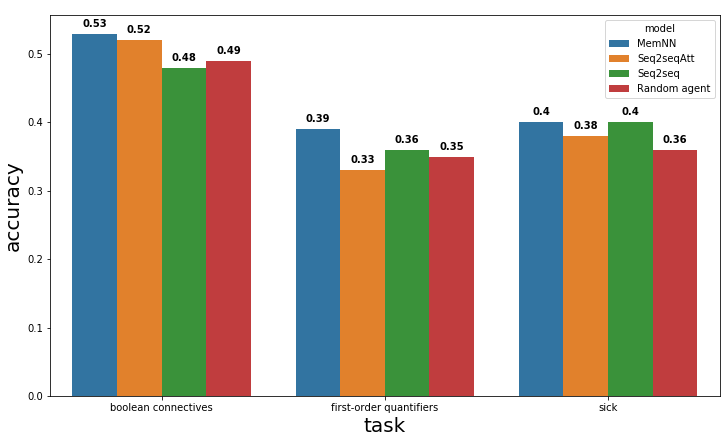
\includegraphics[width=10.0cm]{img/comparative_results.png}
% \captionof{figure}{Test accuracy for the Entailment-QA tasks}
\end{center}

Their overall performance is only slightly better when compared to the random agent. For example, when we look at the memory model, the model that often  outperform the seq2seq model on QA tasks \cite{WestonBCM15}, we can see that regarding tasks 1 and 2 there is an overfitting problem: the model shows high accuracy on the train dataset (75$\%$ accuracy on task 1, and 86$\%$ accuracy on task 2) as can be seen in Figure 2. But when we take a closer look at the confusion matrix of the test data, Figure 3, the results are not impressive.\footnote{All the experiments and the respective results are available on GitHub: \url{https://github.com/felipessalvatore/DialogGym}.}
  

\begin{center}
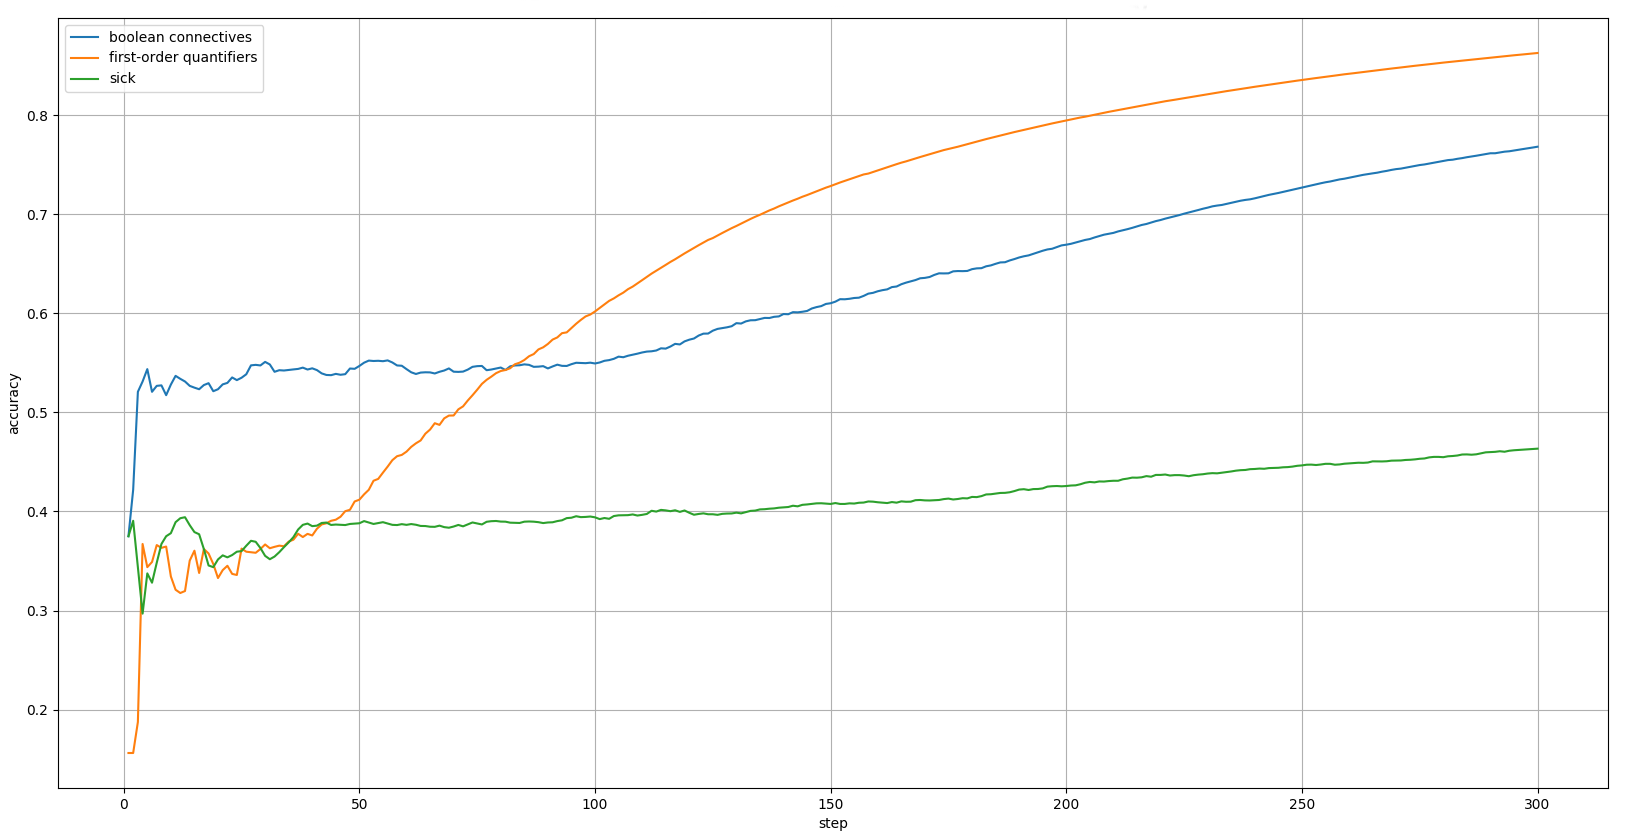
\includegraphics[width=10.0cm]{img/training_acc_EntailQA_mem.png}
% \captionof{figure}{Training accuracy for the memory network}
\end{center}


\begin{center}
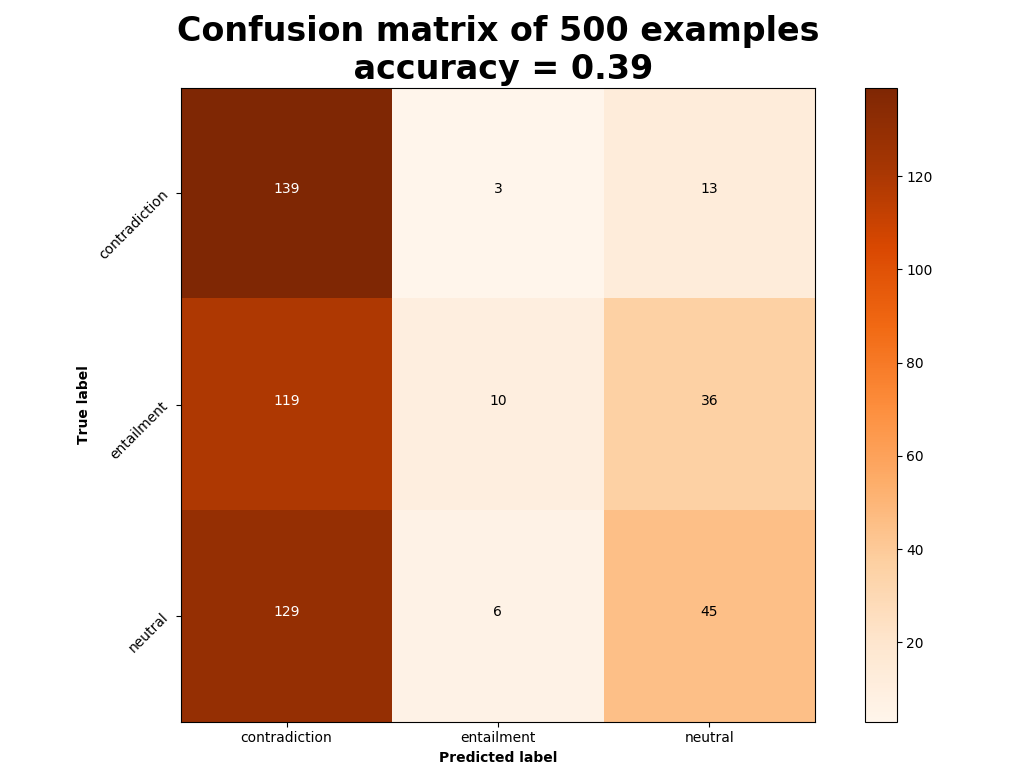
\includegraphics[width=10.0cm]{img/cm_mem_EntailQA2.png}
% \captionof{figure}{Confusion matrix for the memory network on task 2}
\end{center}


\section{KDD comments}
The paper presents a high quality and very interesting research. The concept of incorporating logic reasoning to boost performance of dialogue agent is very promising and employed by the authors in a novel way. The paper is focused on logical reasoning, the area that is often neglected by Conversational AI developers. Splitting the analysis for synonymy, antinomy, hypernymy and active or passive voice is hard to find in recent academic literature. These features make it an outstanding paper.

The Entailment-QA analysis of Neural Network dialog systems on 11000 questions provides interesting results. The fact that the overall accuracy is below 50$\%$ in many cases, points out a significant issue in the current phase of conversational AI. My only concern is that the methods of the research fall outside of Artificial Intelligence (AI) / Machine Learning (ML) domain which makes the paper less relevant to the workshop.

The paper is focused on specific issues of Conversation AI, in particular on complex semantic relationships. The paper is not covering machine learning aspects of Conversation AI. Instead the authors discuss a rule-based approach in more details. The paper would be a good fit for a workshop focused on rule-based methods in Conversational AI and for a workshop focused on automatic testing methods for chatbots. Due to the limitations on the number of accepted papers, this high quality paper might not make it to the short list. I would encourage the authors to proceed with their efforts to publish the paper elsewhere or come back next time when the workshop will have enough bandwidth.
\chapter{Future Steps}
\label{ch04:FutureSteps}

The previous chapters resume what we have done so far: we grasp the theoretical framework to formulate this NLP problem; we reviewed the literature on dialog generation; we built a software workbench to perform different experiments; and we have isolated a specific problem not sufficiently not addressed in the literature: logical reasoning for dialog agents.

In July we will present this work at one summer school organized by the company DeepMind in Europe \url{https://tmlss.ro/} and so we expect to gather more feedback.

To address our research proposal we decided to formulate the following next steps:

\begin{itemize}
\item Apply regularization strategies on the available models to overcome the reported overfitting problem. 
\item Finish the Entailment-QA corpus to have a fine grain analysis of the result that we are seeing on the SICK corpus.
\item Explore the different extensions for all mentioned models.
\item Explore new models not mentioned here, like Dynamic Memory Networks \cite{KumarISBEPOGS15} and the models using the Memory Attention and Composition (MAC) cell \cite{Manning18}.
\item There is a different literature that frames the dialog problem as an MDP (Markovian Decision Process) and a POMDP (Partially Observable Markovian Decision Process) applying different techniques of reinforcement learning (a recent example is \cite{Li:2016}). It is fruitful to investigate if these techniques can help our research.
\item One of the main focused here is model comparison. It would be fruitful if we could use the available literature  on the theory of comparing models (e.g.,  \cite{BenavoliCDZ17}) to refine our analysis.
\end{itemize}


\section{Work Plan}
\label{sec:work-plan}

Here, we use a visual tool to display the scheduling of future and past activities. This serve as a sanity check to verify if the
proposed goals can be realistically achieved.

\begin{table}[ht!]
  \center
  \begin{tabular}{|c|c|c|c|c|c|c|c|c|c|}\hline
    & \multicolumn{2}{c|}{2016} & \multicolumn{2}{c|}{2017} & \multicolumn{2}{c|}{2018} & \multicolumn{2}{c|}{2019} & \multicolumn{1}{c|}{2020} \\ \cline{2-10}
    \raisebox{1.5ex}{Activity} & 1st & 2nd & 1st & 2nd & 1st & 2nd & 1st & 2nd & 1st \\ \hline \hline
    Courses & \cellcolor{green!45} & \cellcolor{green!45} & \cellcolor{green!45}  & \cellcolor{green!45}  &  &  & & & \\ \hline
    Teaching Assist. (PAE) & & &  &  &\cellcolor{green!45}  &  & & & \\ \hline
    Bibliographic Review & \cellcolor{green!45} & \cellcolor{green!45} & \cellcolor{green!45} & \cellcolor{green!45} & \cellcolor{green!45} & &  &  & \\ \hline 
    Software Implementation & & & & \cellcolor{green!45} &\cellcolor{green!45}  & \cellcolor{blue!45} &\cellcolor{blue!45}&\cellcolor{blue!45}& \\ \hline
    Qualification Writing & & & & & \cellcolor{green!45} & &  & & \\ \hline
    Qualification Exam & & & & & \cellcolor{green!45} & & & & \\ \hline
    Finishing Entailment-QA task & & & & & & \cellcolor{blue!45} &  & & \\ \hline
    Improve Training & & & & & & \cellcolor{blue!45} &  & & \\ \hline
    Densemap - Scattering & & & &  & & \cellcolor{blue!25} & &  & \\ \hline
    Active Learning Tool & & & &  & &  & \cellcolor{blue!25} &  & \\ \hline
    Data Augmentation Methods & & & &  & &  & & \cellcolor{blue!25} & \\ \hline
    %Paper Writing & & & & \cellcolor{green!25} & \cellcolor{green!25} & \cellcolor{blue!25} & & \cellcolor{blue!25} & \\ \hline
    Thesis Writing & & & & & & & & \cellcolor{blue!25} & \\ \hline
    Thesis Defense & & & & & & & & & \cellcolor{blue!25}  \\ \hline
  \end{tabular}
  \caption{Schedule for the PhD program. Completed activities are shown in green, while future activities are in blue.}
  \label{tab:schedule}
\end{table}

\bibliography{my_references}
\bibliographystyle{abbrv}

\end{document}


